\documentclass{TIJMUjiaoanLL}
\pagestyle{empty}

\begin{document}

\kecheng{分子生物计算}
\neirong{绪论 \ / 第1章}
\jiaoshi{伊现富}
\zhicheng{讲师}
\riqi{2019年8月28日10:00-11:40}
\duixiang{生物医学工程与技术学院2017级生信班(本)}
\renshu{28}
\fangshi{理论讲授}
\xueshi{2}
\jiaocai{Perl语言在生物信息学中的应用——基础篇}

\firstHeader
\maketitle
\thispagestyle{empty}

\mudi{
\begin{itemize}
  \item 掌握:分子生物学的基础知识;Markdown的基本语法。
  \item 熟悉:格式转换工具pandoc的使用方法。
  \item 了解:生物信息学和计算机科学的概况;生物信息学中常用的编程语言。
  \item 自学:Markdown的扩展语法;使用Markdown进行可重复性研究。
\end{itemize}
}

\fenpei{
\begin{itemize}
  \item (5')引言与导入:回顾已经学习的生物学基础知识。
  \item (40')学科简介:回顾分子生物学的基本知识,介绍生物信息学和计算机科学,比较生物信息学中常用的编程语言。
  \item (40')Markdown标记语言:介绍Markdown,讲解其基本语法与扩展语法,演示Markdown在可重复性研究中的应用以及其格式的转换。
  \item (5')总结与答疑:总结授课内容中的知识点与技能,解答学生疑问。
\end{itemize}
}

\zhongdian{
\begin{itemize}
  \item 重点:Markdown的基本语法。
  \item 难点:Markdown的基本语法。
  \item 解决策略:通过实例演示帮助学生理解、记忆。
\end{itemize}
}

\waiyu{
\vspace*{-10pt}
\begin{multicols}{2}
  生物信息学(bioinformatics)

  分子生物学(molecular biology)

  计算机科学(computer science)

  在活体内(\textit{in vivo})

  在玻璃中(\textit{in vitro})

  在硅之中(\textit{in silico})
\end{multicols}
\vspace*{-10pt}
}

\fuzhu{
\begin{itemize}
  \item 多媒体:生物信息学的研究领域,分子生物学和计算机科学的发展简史,编程语言的比较。
  \item 板书:分子生物学中的中心法则,Markdown的基本语法。
  \item 演示:Markdown在可重复性研究中的应用,格式转换工具pandoc的使用方法。
\end{itemize}
}

\sikao{
\vspace*{-10pt}
\begin{multicols}{2}
\begin{itemize}
  \item 生物信息学是哪些学科的交叉学科?
  \item 生物信息学需要哪些基本的知识和技能?
  \item DNA的碱基组成是什么?和RNA有何不同?
  \item 列举20种氨基酸的三字母和单字母缩写。
  \item 列举常见的存储DNA序列和蛋白质结构的数据库。
  \item 解释\textit{in vivo}、\textit{in vitro}和\textit{in silico}的含义。
  \item 列举生物信息学中常用的编程语言。
  \item 如何使用Markdown实现常见的文本样式?
  \item 如何把Markdown转换成其他常见的格式?
\end{itemize}
\end{multicols}
\vspace*{-10pt}
}

\cankao{
\begin{itemize}
  \item Beginning Perl for Bioinformatics, James Tisdall, O'Reilly Media, 2001.
  \item Perl语言入门(第六版),Randal L. Schwartz, brian d foy \& Tom Phoenix著,盛春\ 译,东南大学出版社,2012。
  \item Mastering Perl for Bioinformatics, James Tisdall, O'Reilly Media, 2003.
  \item 维基百科等网络资源。
\end{itemize}
}

\firstTail

\newpage
\otherHeader

\begin{enumerate}
  \item 引言与导入(5分钟)
    \\回顾生物学的基本知识:孟德尔遗传定律,DNA双螺旋结构,人类基因组计划,……
  \item 学科简介(40分钟)
    \begin{enumerate}
      \item 生物信息学
	\begin{itemize}
    \item 交叉学科:生物学/(医学)、计算机科学、数学(统计学)
	  \item 知识/技能:生物学/(医学)、计算机编程、数理统计
	  \item 研究内容:计算(算法、软件、数据库),应用(序列分析、功能分析、结构分析)
	\end{itemize}
      \item 分子生物学
	\begin{itemize}
	  \item 中心法则:DNA$\rightarrow$RNA$\rightarrow$蛋白质
	  \item 核酸:DNA(A、C、G、T),RNA(A、C、G、U)
	  \item 蛋白质:氨基酸$\rightarrow$多肽,一级结构$\rightarrow$二级结构$\rightarrow$三级结构$\rightarrow$四级结构
	  \item 数据库:GenBank,PDB
	\end{itemize}
      \item 计算机科学
	\begin{itemize}
	  \item 术语:\textit{in vivo}(生物活体内),\textit{in vitro}(生物活体外),\textit{in silico}(进行于电脑中)
	\end{itemize}
      \item 编程语言\textcolor{red}{(进行可视化比较,基于Bioinformatics Career Survey 2008/2010进行讲解)}
	\begin{itemize}
	  \item 计算机编程语言:C、C++、C\#、Java、Python、Perl、Ruby、JavaScript、PHP、……
	  \item 生物信息学常用编程语言:Perl(1987)、Python(1991)、Ruby(1995)、Java(1995)
	  \item 生物信息学专用:BioPerl、Biopython、BioRuby、BioJava
	\end{itemize}
    \end{enumerate}
  \item Markdown标记语言(40分钟)
    \begin{enumerate}
      \item \textcolor{red}{【重点、难点】}基本语法\textcolor{red}{(逐一进行演示)}
	\begin{figure}[h]
	  \centering
	  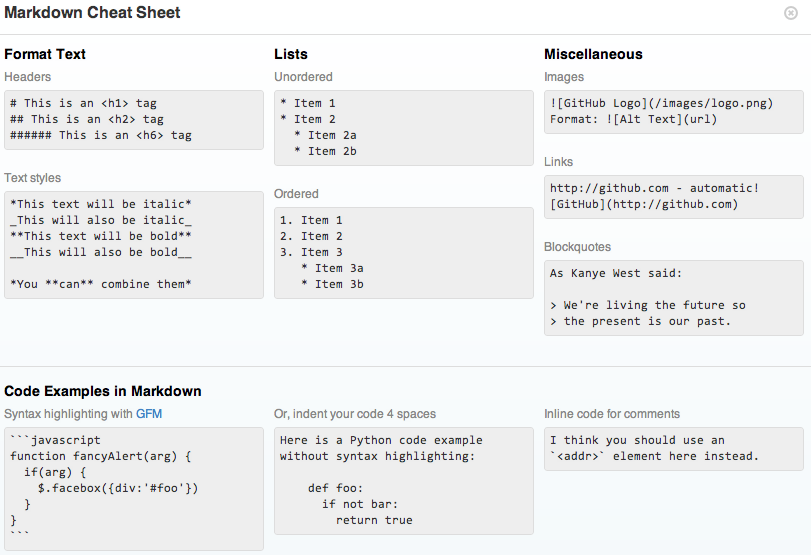
\includegraphics[width=0.9\textwidth]{c1_markdown_cheatsheet_02.png}
	\end{figure}
      \item 扩展语法:目录、标签、表格、公式、流程图、……
      \item 可重复性研究\textcolor{red}{(展示实例)}:$R+Markdown+knitr$(RStudio)
      \item 格式转换\textcolor{red}{(进行操作演示)}:pandoc
    \end{enumerate}

\otherTail
\newpage
\otherHeader

  \item 总结与答疑(5分钟)
    \begin{enumerate}
      \item 知识点
	\begin{itemize}
	  \item 生物信息学:交叉学科、多种技能、领域宽泛
	  \item 分子生物学:DNA、RNA、蛋白质
	  \item 计算机科学:\textit{in vivo}、\textit{in vitro}、\textit{in silico}
	  \item 编程语言:Perl、Python、Ruby、Java
	  \item Markdown语法:标题、文本样式、列表、链接、引用、插入代码、……
	  \item Markdown相关:knitr、pandoc
	\end{itemize}
      \item 技能
	\begin{itemize}
	  \item 熟练使用Markdown撰写文档
	  \item 使用pandoc转换文档格式
	\end{itemize}
    \end{enumerate}
\end{enumerate}

\otherTail

\end{document}
